\documentclass[
	a4paper,
	oneside,
	BCOR = 10mm,
	DIV = 12,
	12pt,
	headings = normal,
]{scrartcl}

%%% Length calculations
\usepackage{calc}
%%%

%%% Support for color
\usepackage{xcolor}
\definecolor{lightblue}{HTML}{03A9F4}
\definecolor{red}{HTML}{F44336}
%%%

%%% Including graphics
\usepackage{graphicx}
%%%

%%% Font selection
\usepackage{fontspec}

\setromanfont{STIX Two Text}[
	SmallCapsFeatures = {LetterSpace = 8},
]

\setsansfont{IBM Plex Sans}[
	Scale = MatchUppercase,
]

\setmonofont{IBM Plex Mono}[
	Scale = MatchUppercase,
]
%%%

%%% Math typesetting
\usepackage{amsmath}

\usepackage{unicode-math}
\setmathfont{STIX Two Math}

\usepackage{IEEEtrantools}
%%%

%%% List settings
\usepackage{enumitem}
\setlist[enumerate]{
	label*      = {\arabic*.},
	leftmargin  = *,
	labelindent = \parindent,
	topsep      = 1\baselineskip,
	parsep      = 0\baselineskip,
	itemsep     = 1\baselineskip,
	noitemsep, % override itemsep
}

\setlist[itemize]{
	label*      = {—},
	leftmargin  = *,
	labelindent = \parindent,
	topsep      = 1\baselineskip,
	parsep      = 0\baselineskip,
	itemsep     = 1\baselineskip,
	noitemsep, % override itemsep
}

\setlist[description]{
	font        = {\rmfamily\upshape\bfseries},
	topsep      = 1\baselineskip,
	parsep      = 0\baselineskip,
	itemsep     = 0\baselineskip,
}

%%%

%%% Structural elements typesetting
\setkomafont{pagenumber}{\rmfamily\upshape}
\setkomafont{disposition}{\rmfamily\bfseries}

% Sectioning
\RedeclareSectionCommand[
	beforeskip = -1\baselineskip,
	afterskip  = 1\baselineskip,
	font       = {\normalsize\bfseries\scshape},
]{section}

\RedeclareSectionCommand[
	beforeskip = -1\baselineskip,
	afterskip  = 1\baselineskip,
	font       = {\normalsize\bfseries\itshape},
]{subsection}

\RedeclareSectionCommand[
	beforeskip = -1\baselineskip,
	afterskip  = 1\baselineskip,
	font       = {\normalsize\bfseries},
]{subsubsection}

\RedeclareSectionCommand[
	beforeskip = -1\baselineskip,
	afterskip  = -0.5em,
	font       = {\normalsize\mdseries\scshape\addfontfeatures{Letters = {UppercaseSmallCaps}}},
]{paragraph}
%%%

%%% Typographic enhancements
\usepackage{microtype}
%%%

%%% Language-specific settings
\usepackage{polyglossia}
\setmainlanguage{ukrainian}
\setotherlanguages{english}
%%%

%%% Captions
\usepackage{caption}
\usepackage{subcaption}

%\DeclareCaptionLabelFormat{closing}{#2)}
%\captionsetup[subtable]{labelformat = closing}

%\captionsetup[subfigure]{labelformat = closing}

\captionsetup[table]{
	aboveskip = 0\baselineskip,
	belowskip = 0\baselineskip,
}

\captionsetup[figure]{
	aboveskip = 1\baselineskip,
	belowskip = 0\baselineskip,
}

\captionsetup[subfigure]{
	labelformat = simple,
	labelformat = brace,
}
%%%

%%% Hyphenated ragged typesetting
\usepackage{ragged2e}
%%%

%%% Table typesetting
\usepackage{booktabs}
\usepackage{longtable}

\usepackage{multirow}

\usepackage{array}
\newcolumntype{v}[1]{>{\RaggedRight\arraybackslash\hspace{0pt}}p{#1}}
\newcolumntype{b}[1]{>{\Centering\arraybackslash\hspace{0pt}}p{#1}}
\newcolumntype{n}[1]{>{\RaggedLeft\arraybackslash\hspace{0pt}}p{#1}}
%%%

%%% Drawing
\usepackage{tikz}
\usepackage{tikzscale}
\usetikzlibrary{positioning}
\usetikzlibrary{arrows.meta} % Stealth arrow tips
%%%

%%% SI units typesetting
\usepackage{siunitx}
\sisetup{
	output-decimal-marker = {,},
	exponent-product      = {\cdot},
	inter-unit-product    = \ensuremath{{} \cdot {}},
	per-mode              = symbol,
}
%%%

%%% Framing code listings
\usepackage{tcolorbox}
\tcbuselibrary{breakable}
\tcbuselibrary{minted}
\tcbuselibrary{skins}

\newtcblisting[
	auto counter, 
	list inside, 
	number within = section,
]{listingpython}[3][]{%
	minted language = python,
	minted style    = bw,
	minted options  = {
		linenos,
		tabsize = 4,
		breaklines,
		breakanywhere,
		fontsize = \footnotesize,
	},
	empty,
	sharp corners,
	coltitle = black,
	borderline horizontal = {1pt}{0pt}{black},
	titlerule = {0.5pt},
	titlerule style = {
		black,
	},
	toptitle = 0.3em,
	bottomtitle = 0.3em,
	before skip      = \intextsep,
	after  skip      = \intextsep,
	title            = {Лістинг \thetcbcounter: #2},
	list entry       = {\protect\numberline{\thetcbcounter}#2},
	left = 0em,
	right = 0em,
	%
	listing only,
	breakable,
	%
	label = {#3},
	%
	#1
}

\newtcbinputlisting[auto counter, list inside, number within = section]{\inputpython}[4][]{%
	minted language = python,
	minted style    = bw,
	minted options  = {
		linenos,
		tabsize = 4,
		breaklines,
		breakanywhere,
		fontsize = \footnotesize,
	},
	empty,
	sharp corners,
	coltitle = black,
	borderline horizontal = {1pt}{0pt}{black},
	titlerule = {0.5pt},
	titlerule style = {
		black,
	},
	toptitle = 0.3em,
	bottomtitle = 0.3em,
	before skip      = \intextsep,
	after  skip      = \intextsep,
	title            = {Лістинг \thetcbcounter: #3},
	list entry       = {\protect\numberline{\thetcbcounter}#3},
	left = 0em,
	right = 0em,
	%
	listing file={#2},
	listing only,
	breakable,
	%
	label = {#4},
	%
	#1
}

% Customize minted
\usepackage{minted}
\setmintedinline{
	style = bw,
	breaklines,
}

% Customize minted line numbers
\renewcommand{\theFancyVerbLine}{\ttfamily\scriptsize\arabic{FancyVerbLine}}

%%%

%%% Links and hyperreferences
\usepackage{hyperref}
\hypersetup{
	bookmarksnumbered = true,
	colorlinks      = false,
	linkbordercolor = red,
	urlbordercolor  = lightblue,
	pdfborderstyle  = {/S/U/W 1.5},
}
%%%

%%% Length adjustment

% Set baselineskip, default is 14.5 pt
\linespread{1.068966} % ~15.5 pt
\setlength{\emergencystretch}{1em}
\setlength{\parindent}{1.5em}
\newlength{\gridunitwidth}
\setlength{\gridunitwidth}{\textwidth / 12}
%%%

%%% Custom commands
\newcommand{\allcaps}[1]{{\addfontfeatures{LetterSpace = 8, Kerning = Off}#1}}
\newcommand{\filename}[1]{\texttt{#1}}
\newcommand{\progname}[1]{\texttt{#1}}
\newcommand{\modulename}[1]{\texttt{#1}}
%%%

%%% Custom math commands
\newcommand{\longvar}[1]{\mathit{#1}}
%%%

\begin{document}

\begin{titlepage}
		\begin{center}
			Міністерство освіти і науки України\\
			Національний авіаційний університет\\
			Навчально-науковий інститут комп'ютерних інформаційних технологій\\
			Кафедра комп'ютеризованих систем управління

			\vspace{\fill}
				Лабораторна робота №5\\
				з~дисципліни «Імітаційне моделювання»\\
				на~тему «Моделювання процесу функціонування системи за принципом~$\Delta t$»\\

			\vspace{\fill}

			\begin{flushright}
				Виконав:\\
				студент \allcaps{ННІКІТ}\\
				групи СП-325\\
				Клокун В.\,Д.\\
				Перевірила:\\
				Марченко Н.\,Б.
			\end{flushright}

			Київ 2019
		\end{center}
	\end{titlepage}

	\section{Мета роботи}
		Ознайомитись з~методами імітаційного моделювання та принципами побудови моделі процесу функціонування системи; побудувати імітайційну модель процесу функціонування системи в часі за принципом~$\Delta t$.

	\section{Хід роботи}
		Для виконання роботи поставлені такі завдання:
		\begin{enumerate}
			\item Побудувати імітаційну модель процесу функціонування системи в часі.
			\item На основі отриманих даних в створеній програмі побудувати траєкторію процесу функціонування системи.
			\item Знайти ймовірність того, що неперервна випадкова величина~$X$ прийме значення, яке належить інтервалу~$[a; b]$.
		\end{enumerate}

		\paragraph{Завдання за варіантом} У резервуар, що містить~$m$~\si{\kilo\gram} солі на~$V_1$~\si{\litre} суміші, кожну хвилину поступає~$v$~\si{\litre} води та витікає~$V_2$~\si{\litre} суміші. Процес концентрації розчину відбувається за законом:
		\begin{IEEEeqnarray*}{rCl}
			x(t) = \frac{V_1 (v - V_2)}{(m + t)^2}.
		\end{IEEEeqnarray*}
		Імітувати процес концентрації розчину в часі з кроком~$\Delta t$, якщо при~$t = 0$ значення~$x=10$. Значення~$\Delta t$ вибирається з інтервалу~$(0; 1)$ за допомогою генератора псевдовипадкових чисел. Визначити, яка кількість солі залишиться в резеруварі через~$t$~хвилин, припускаючи, що суміш миттєво змішується. Значення змінних~$V_1$, $V_2$, $v$ та~$m$ вводяться користувачем.

		Під час виконання роботи була розроблена імітаційна модель для виконання поставлених завдань і реалізована у вигляді відповідного програмного засобу (ліст.~\ref{lst:full-solution}). Реалізований програмний засіб був запущений на~моделювання і~надавав стабільний і~очікуваний результат~(рис.~\ref{fig:program_scr}). В результаті програма будує графік траєкторії процесу функціонування системи~(рис.~\ref{fig:pmf}).

		\begin{figure}[!htbp]
			\centering
			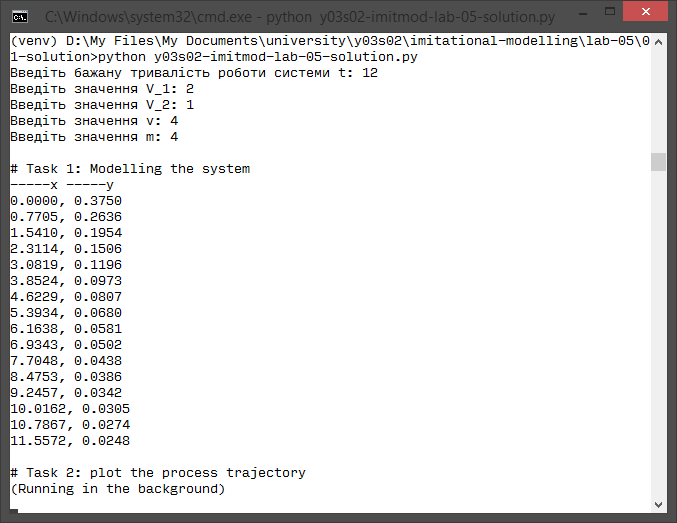
\includegraphics[height = 14\baselineskip]{./assets/y03s02-imitmod-lab-04-p00.png}
			\caption{Результат роботи програми: вікно терміналу}
			\label{fig:program_scr}
		\end{figure}
		
		\begin{figure}[!htbp]
			\centering
			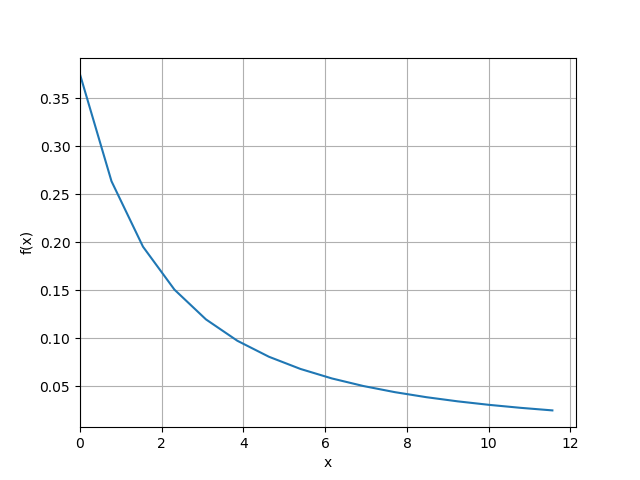
\includegraphics[height = 14\baselineskip]{./assets/y03s02-imitmod-lab-04-p01.png}
			\caption{Графік траєкторії процесу функціонування системи}
			\label{fig:pmf}
		\end{figure}

		\section{Висновок}
			Виконуючи дану лабораторну роботу, ми ознайомились з~методом оберненої функції імітації неперервних випадкових величин; побудували імітаційну модель отримання системи неперервних випадкових величин (СНВВ).

		\appendix
		\section{Повний початковий код програмної реалізації}
		\label{sec:full-listing}
			\begin{listingpython}[toprule = 0pt, bottomrule = 0pt]{Повний початковий код програмної реалізації}{lst:full-solution}
#!/usr/bin/env python3
# -*- coding: utf-8 -*-
import random
import multiprocessing as mp
import matplotlib.pyplot as plt


class Model(object):
    """ A class that represets a process model
    """

    def __init__(self, functional_law, delta_t_min, delta_t_max,
                 delta_t=None, **kwargs):
        """
        :param functional_law: A function that describes how a model
            behaves in time
        :type functional_law: func
        :param delta_t_min: lower bound for randomly generating delta_t
        :type delta_t_min: float
        :param delta_t_max: upper bound for randomly generating delta_t
        :type delta_t_max: float
        :param delta_t: explicit delta_t value. Overrides generated one.
        :type delta_t: float
        """
        # The functional law itself
        self.functional_law = functional_law
        # Variables neccessary for the functional_law to be computed
        self.functional_law_vars = kwargs
        # Time step
        self.delta_t = random.uniform(delta_t_min, delta_t_max)
        # If delta_t is explicitly passed, override it
        if delta_t:
            self.delta_t = delta_t

    def run(self, t):
        """
        Run the model at time point "T"

        :param t: time point value
        :type t: float

        :return: time point t and the value of a system in time point t
        :rtype: tuple
        """
        return t, self.functional_law(**self.functional_law_vars, t=t)

    def run_for(self, time):
        """
        A generator function that runs a model for a given duration `time`

        :param time: time duration how long a model should be run
        :type time: float
        """
        t = 0
        while t < time:
            yield self.run(t)
            t += self.delta_t


def split_list_of_points(lofp):
    """ Splits a list of points of form [(x1, y1), (x2, y2), (x3, y3), ...]
    into [x1, x2, x3, ...], [y1, y2, y3, ...]
    """
    lx, ly = zip(*lofp)
    return lx, ly


def print_table(t, colh1='x', colh2='y'):
    print('{:->6} {:->6}'.format(colh1, colh2))
    for x, y in t:
        print('{:02.4f}, {:02.4f}'.format(x, y))


def plot_func(x, y, xlabel='x', ylabel='f(x)'):
    fig = plt.figure(1)

    ax = fig.add_subplot(111)
    ax.plot(x, y)
    ax.set_xlabel(xlabel)
    ax.set_ylabel(ylabel)
    ax.set_xlim(0.0, None)
    plt.grid()
    plt.show()
    return


def main():
    # Declare the function described in the task
    def f(t, V_1, V_2, v, m): return (V_1 * (v-V_2)) / (m+t)**2

    # Read the time duration
    t = float(input('Введіть бажану тривалість роботи системи t: '))

    # Read the needed parameters from stdin
    V_1 = float(input('Введіть значення V_1: '))
    V_2 = float(input('Введіть значення V_2: '))
    v = float(input('Введіть значення v: '))
    m = float(input('Введіть значення m: '))

    # Run the system
    # Pass every needed variable as a keyword argument
    print('\n# Task 1: Modelling the system')

    sys = Model(f, 0, 1, V_1=V_1, V_2=V_2, v=v, m=m)
    simulation_table = [x for x in sys.run_for(time=t)]
    print_table(simulation_table)
    x, y = split_list_of_points(simulation_table)

    # Task 2: Plot process trajetory
    print('\n# Task 2: plot the process trajectory'
          '\n(Running in the background)')

    p = mp.Process(target=plot_func, args=(x, y))
    p.start()


if __name__ == '__main__':
    main()
			\end{listingpython}

\end{document}

